% !TeX root = main.tex
\lecture{15}{Mon 09 Mar 2026 11:00}{Ampere's Law}

\section{Biot-Savat: Complex Loops Continued}
Continuing from the end of last lecture, we found by symmetry that the $yz$ components cancel, leaving only an $x$ component for any point $P$ along the x-axis.

\begin{figure}[H]
    \centering
    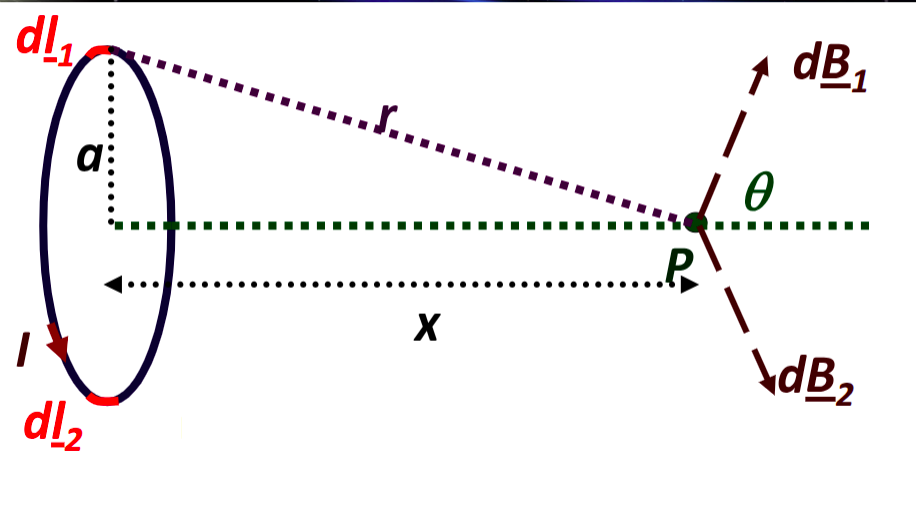
\includegraphics[width=0.75\textwidth]{figures/lec14-07.png}
     \caption{}
\end{figure}

\begin{figure}[H]
    \centering
    
\includegraphics[width=0.75\textwidth]{figures/lec15-01.png}
     \caption{}
\end{figure}

Taking magnitudes (and noting that $\hat{r}$ is a unit vector):
\[
    \delta B = \frac{\mu_0 I}{4 \pi r^2} \delta l
\]


Resolving into the x-direction, we get that:
\[
    \delta B_{x} = \frac{\mu_0 I}{4 \pi r^2} \delta l \cos \theta \tag{1}
\]

And as we have a right angled triangle:
\[
    r^2 + a^2 + x^2 \tag{2}
\]
\[
    \cos \theta = \frac{a}{r} \implies \cos \theta = \frac{a}{\left(a^2 + x^2\right)^{(1/2)}} \tag{3}
\]

Inserting 2 and 3 into 1:
\[
    \delta B_x = \frac{\mu_0 I}{4 \pi} \times \frac{a}{\left(a^2 + x^2\right)^{(3/2)}} \delta l
\]
\[
    B_x = \frac{\mu_0 I}{4 \pi} \times \frac{a}{\left(a^2 + x^2\right)^{(3/2)}} \oint \delta l
\]
\[
    B_x = \frac{\mu_0 I}{4 \pi} \times \frac{a}{\left(a^2 + x^2\right)^{(3/2)}} 2 \pi a
\]
\[
    B_x = \frac{\mu_0 I}{2} \frac{a^2}{\left(a^2 + x^2\right)^{(3/2)}}
\]

Taking limits, we can observe that at the centre of the loop (where $x=0$):
\[
    B_0 =  \frac{\mu_0 I}{2} \frac{a^2}{\left(a^2\right)^{(3/2)}}= \frac{\mu_0 I}{2a}
\]

And when $x\gg a$, we have:
\[
    B_x = \frac{\mu_0 I a^2 }{2x^3}
\]

However, we can simplify using the magnetic dipole moment $\mu_m = I \times \text{area} = I \pi a^2$, hence:
\[
    B_x = \frac{\mu_0}{4 \pi} \frac{2 \mu_m}{x^3}
\]

This is strikingly similar for the expression for an electric dipole:
\[
    E_x = \frac{1}{4 \pi \epsilon_0} \frac{2p}{x^3}
\]


\section{E- and B-Fields}
We have already determined the following, for E- and B-fields respectively:
\[
    \int_S \underline{E} \cdot d \underline{S} = \frac{Q}{\epsilon_0} \tag{E}
\]
\[
    \int_S \underline{B} \cdot d \underline{S} = 0 \tag{B}
\]

We also know that the E-field is conservative, hence no work is done if a charge returns to its original position:
\[
    \oint \underline{E} \cdot d \underline{l} = 0
\]

Is there an equivalent of this for B-fields?

Consider a circiular path of a B-field created around an infinite line of current at radial distance $r$. By symmetry, $\underline{B}$ and $d \underline{l}$ are parallel, and are constant for a fixed $r$. Hence:
\[
    \oint \underline{B} \cdot d \underline{l} = \oint B dl = B \oint dL = B 2 \pi r
\]

We have also determined that:
\[
    B = \frac{\mu_0 I}{2 \pi r} \implies \oint \underline{B} \cdot d \underline{l} = B 2 \pi r = \frac{\mu_0 I}{2 \pi r} \times 2 \pi r = \mu_0 I
\]


This gives us Ampere's Law:
\[
    \boxed{\oint \underline{B} \cdot d \underline{l} = \mu_0 I_\text{enclosed}}
\]

\subsection{Example}
Consider a long solid cylinder carrying a uniformly distributed current. The cylinder has radius $R$ and length
